
\documentclass[a4paper]{article}
\usepackage[a4paper,top=2cm,bottom=2cm,left=2cm,right=2cm,marginparwidth=2cm]{geometry}
\usepackage{lmodern}
\usepackage{listings}
\usepackage{amsmath}
\usepackage{amssymb}
\usepackage{bm}
\usepackage{textpos} % package for the positioning
\usepackage{tcolorbox}
\usepackage{pgf, tikz}
\usepackage{url}
\usetikzlibrary{arrows, automata}

\setlength{\parindent}{0em}
\setlength{\parskip}{0.3em}

\usepackage{textcomp}
\begin{document}

\lstset{language=Python,upquote=true}

\setlength{\leftskip}{20pt}
\title{Lab 5 Exercise - A little Linear Regression}
\author{Jonathon Hare (jsh2@ecs.soton.ac.uk)}

\maketitle

% \begin{abstract}
% \end{abstract}
% \tableofcontents

This is the exercise that you need to work through \textbf{on your own} after completing the forth lab session. You'll need to write up your results/answers/findings and submit this to ECS handin as a PDF document along with the other lab exercises near the end of the module (1 pdf document per lab). 

We expect that you \textbf{will use no more than one side} of A4 to cover your responses to \emph{this} exercise. This exercise is worth 5\% of your overall module grade.

\section{An initial attempt}\label{init}

In the lab exercise you built and trained a couple of CNNs for image classification. Your now going to try something different and build some CNNs for image-to-vector regression task - in particular you're going to implement a network that takes an image of a scatter plot, and predicts the parameters of the line of best fit.

\begin{figure}[h!]
\center
	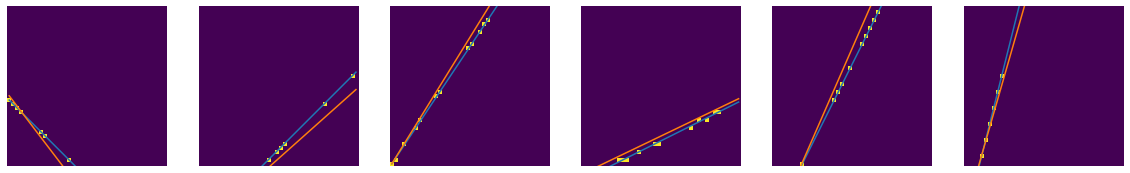
\includegraphics[width=0.9\textwidth]{plots.png}
\end{figure}

The following code is used to generate the datasets for this task (get it in a useable form here: \url{https://gist.github.com/jonhare/73a59dcc5416729548a086a983e81f07}):

\begin{lstlisting}[language=Python]
import torch
from torchvision import transforms
from torch.utils.data import Dataset

class MyDataset(Dataset):
  def __init__(self, size=5000, dim=40, random_offset=0):
        super(MyDataset, self).__init__()
        self.size = size
        self.dim = dim
        self.random_offset = random_offset

  def __getitem__(self, index):
      if index >= len(self):
          raise IndexError('{} index out of range'.format(self.__class__.__name__))
      
      rng_state = torch.get_rng_state()
      torch.manual_seed(index + self.random_offset)
      
      while True:
        img = torch.zeros(self.dim, self.dim)
        dx = torch.randint(-10,10,(1,),dtype=torch.float)
        dy = torch.randint(-10,10,(1,),dtype=torch.float)
        c = torch.randint(-20,20,(1,), dtype=torch.float)
        
        params = torch.cat((dy/dx, c))
        xy = torch.randint(0,img.shape[1], (20, 2), dtype=torch.float)
        xy[:,1] = xy[:,0] * params[0] + params[1]

        xy.round_()
        xy = xy[ xy[:,1] > 0 ]
        xy = xy[ xy[:,1] < self.dim ]
        xy = xy[ xy[:,0] < self.dim ]

        for i in range(xy.shape[0]):
          x, y = xy[i][0], self.dim - xy[i][1]
          img[int(y), int(x)]=1
        if img.sum() > 2:
          break

      torch.set_rng_state(rng_state)
      return img.unsqueeze(0), params

  def __len__(self):
      return self.size
  
train_data = MyDataset()
val_data = MyDataset(size=500, random_offset=33333)
test_data = MyDataset(size=500, random_offset=99999)
\end{lstlisting}

\begin{tcolorbox}[title=1.1 A simple CNN baseline (2 marks)]
Implement the following CNN model, and train it using Adam (default parameters) for 100 epochs (use a GPU and be prepared to wait 6 or 7 minutes!). Use shuffled batches of 128 items. State the loss function you're using. \textbf{Comment} on the performance of the model.

\begin{lstlisting}
Convolution2D, channels=48, size=3x3, stride=1, padding=1
ReLU
Linear, 128 outputs
ReLU
Linear, 2 outputs
\end{lstlisting}
\end{tcolorbox}

\section{A second attempt}\label{second}

Clearly the CNN implemented in Section~\ref{init} has many parameters in its final hidden layers. One common way of reducing this is to use Global Max Pooling to flatten the feature maps into a vector (called \verb|AdaptiveMaxPool2d| in PyTorch).

\begin{tcolorbox}[title=2.1 A simple CNN with global pooling (1 mark)]
Implement the following CNN model, and train it using Adam (default parameters) for 100 epochs. Use shuffled batches of 128 items. \textbf{Comment} on the model performance.

\begin{lstlisting}
Convolution2D, channels=48, size=3x3, stride=1, padding=1
ReLU
Convolution2D, channels=48, size=3x3, stride=1, padding=1
ReLU
Global Max Pool
Linear, 128 outputs
ReLU
Linear, 2 outputs
\end{lstlisting}
\end{tcolorbox}

\section{Something that actually works?}\label{final}
The two models so far likely have a few issues. We're now going to try and fix this.

\begin{tcolorbox}[title=3.1 Let's regress (2 marks)]
Modify the model from Section~\ref{second} as follows:
\begin{enumerate}
	\item Modify the number of input channels to the first convolutional layer to be 3 instead of 1
	\item In the forward pass, before the first convolution, modify the input, \verb|x|, using the following code:
	\begin{lstlisting}[language=Python]
    idxx = torch.repeat_interleave(
        torch.arange(-20,20, dtype=torch.float).unsqueeze(0) / 40.0, 
        repeats=40, dim=0).to(x.device)
    idxy = idxx.clone().t()
    idx = torch.stack([idxx, idxy]).unsqueeze(0)
    idx = torch.repeat_interleave(idx, repeats=x.shape[0], dim=0)
    x = torch.cat([x, idx], dim=1)
	\end{lstlisting}
\end{enumerate}
Train the modified model using Adam (default parameters) for 100 epochs. Use shuffled batches of 128 items. \textbf{Comment} on the model performance. \textbf{Describe} the rationale for the modification that was made.
\end{tcolorbox}
\end{document}
